%%%%%%%%%%%%%%%%%%%%%%%%%%%%%%%%%%%%%%%%%%%%%%%%%%%%%%%%%%%%
% Pedro Brandao's trial to get a template for thesis for students
% Used the upthesis from Fernando Silva (see upthesis).
% See also the packages file.
% 2014/07/07 First draft
% 2014/07/21 
%  pbrandao: added the list of listings (it should produce portuguese name if
%           babel is set to portuguese, see packages.tex). Changed usepackage of babel
%           to be before input packages.tex to allow test

%
%%%%%%%%%%%%%%%%%%%%%%%%%%%%%%%%%%%%%%%%%%%%%%%%%%%%%%%%%%%%
% LTeX: language=portuguese

% makes all pages the height of the text on that page. No extra vertical space is added.
\raggedbottom 
% setting it to report will remove the blank pages before each chapter
\documentclass[11pt,a4paper,twoside]{book}


%%%%%%%%%%%%%%%%%%%%%%%%%%%%%%%%%%%%%%%%%%%%%%%%%%%%%%%%%%%%
%%%   Packages that need to be configured for the thesis
%%%%%%%%%%%%%%%%%%%%%%%%%%%%%%%%%%%%%%%%%%%%%%%%%%%%%%%%%%%%

% Language settings
% use UKenglish for UK or leave blank for US English
% it will also change the names for some of the chapters (list of tables, figures, content,
%\usepackage[UKenglish]{babel}
%\usepackage[portuguese]{babel}
% If you have multiple languages (as in this text) you can use both, leaving last the main one.
% Then you can use 
% \begin{otherlanguage}{UKenglish}
% text in other language, UKEnglish in this case
% \end{otherlanguage}
\usepackage[UKenglish]{babel}


%%%%%%%%%%%%%%%%%%%%%%%%%%%%%%%%%%%%%%%%%%%%%%%%%%%%%%%%%%%%
%%%   Packages uses language definitions
% see file below for more packages and settings
%%%%%%%%%%%%%%%%%%%%%%%%%%%%%%%%%%%%%%%%%%%%%%%%%%%%%%%%%%%%
\usepackage{upthesis}

\usepackage{algorithm}
\usepackage{algpseudocode}

% the bibliography file
\addbibresource{refs.bib}


%% Definitions for acronyms
\newcommand*\acronymbiggest{HTTP} % defines the biggest Acronym used to define the column size



\usepackage[
%backref={section},
%pagebackref, % for getting references to the page where the citation is (in the biblio), note that biblatex above also has this
pdfpagelabels=false
]{hyperref}
\hypersetup{pdftitle={Test}, %nao suporta acentos
   pdfkeywords ={palavras chave},
   pdfsubject = {assunto},
	bookmarksnumbered=true,
   pdfauthor ={Your name}, % see other options on manual (can be page) needs empty line on bibitem
   plainpages=false, 
   pdfborder={0 0 0},
   colorlinks,%colorlinks=false,
   breaklinks=true,
	%hyperindex=true 	% Makes the page numbers of index entries into hyperlinks. Relays on unique page anchors (pageanchor) 
% see for colors http://mirror.ctan.org/macros/latex/contrib/xcolor/xcolor.pdf
   linkcolor=Sepia, %MidnightBlue,% BlueViolet,%Sepia, % Color for normal internal links.
   %anchorcolor=black,% Color for anchor text.
   citecolor=RedViolet,% Color for bibliographical citations in text.
   %filecolor=cyan% Color for URLs which open local files.
   %menucolor=red% Color for Acrobat menu items.
   %runcolor=filecolor% Color for run links (launch annotations).
   urlcolor=NavyBlue% Color for linked URLs.
}
%use the same style for \url as the text
% from http://en.wikibooks.org/wiki/LaTeX/Hyperlinks#Customization
\urlstyle{same}

\usepackage{tikz}
\usetikzlibrary{automata,positioning}


\begin{document}

\title{Thesis title}
%% The following is not currently being used.
% Part of the coverp in upthesis.sty
% \submitionplace{Tese submetida à Faculdade de Ciências da \\
%   Universidade do Porto para obtenção do grau de Mestre \\ 
%   em Ciência de Computadores}
% \author{Nome do autor}
% \department{Departamento de Ciência de Computadores \\ Faculdade de
%   Ciências da Universidade do Porto}
% \submitdate{Setembro 2015}


\beforepreface%

\prefacesection{Abstract}
Regular expressions (\emph{regex}) are a foundational tool in modern software, widely used for string matching, input validation, and text parsing. Despite their utility, improperly constructed regular expressions can introduce serious security vulnerabilities. One of the most critical threats is the Regular Expression Denial of Service (\emph{ReDoS}) attack, in which carefully crafted inputs cause the regex engine to perform excessive and redundant processing. This results in dramatic slowdowns or even complete unresponsiveness of the system. ReDoS poses a significant risk to web applications, APIs, and other input-facing systems, where user-controlled input is matched against vulnerable patterns.

In this work, we propose a system to address ReDoS by transforming regular expressions into a modified \emph{position automata}, a form of nondeterministic finite automaton (NFA) that tracks the exact start and end positions of all matches within an input string. This structure enables a matching function that computes \emph{all} match positions, including overlapping ones, without relying on backtracking. By exhaustively and efficiently exploring the automaton's transitions, our approach avoids the exponential blowup typical of vulnerable engines, while preserving a somewhat full regex expressiveness.

Furthermore, we also review and compare this approach with existing solutions present in state-of-the-art programming languages and libraries, such as \emph{RE\#}.
\textbf{Palavras-chave:} regular expressions, ReDoS, position automata, nondeterministic finite automata, pattern matching.

\prefacesection{Resumo}
O teu resumo COOL, its me TEST WOWIEESSS

\textbf{Palavras-chave:} palavra, chave..


\prefacesection{Acknowledgements}

First of all, I would like to thank my family, etc, etc
\dedicationpage{Dedico à minha mãe \ldots}



% end of thesis preamble
\afterpreface%

%% main tex here
%% By putting the chapter names here, one can just comment the content in the chapters 
%% and produce a pdf with the correct chapter number.
%% If you want further configurability you can use subfiles package
%% https://www.ctan.org/pkg/subfiles

\chapter{Introduction}\label{chap:intro}

%https://www.usenix.org/system/files/sec22-turonova.pdf
%https://arxiv.org/abs/2407.20479
%https://www.regular-expressions.info/catastrophic.html

Regular expressions are a powerful and ubiquitous tool in software development, enabling concise and expressive definitions of complex text patterns. However, their utility comes with a hidden cost: when implemented naively or misused, certain regular expression constructs can expose systems to catastrophic performance degradation. This vulnerability, known as Regular Expression Denial of Service (ReDoS), arises particularly in backtracking-based matching engines and has been responsible for real-world outages across major platforms. 

This chapter introduces the ReDoS problem by first providing foundational background on regular expression engines and their operational behavior. It then outlines the nature of ReDoS vulnerabilities, illustrating their practical impact through two real-world case studies. Finally, it discusses the reasons for continued reliance on legacy engines despite known risks. By establishing the technical and practical motivations behind this research, this chapter sets the stage for the proposed approach introduced in the subsequent chapters.

\section{Background}
Regular expressions are a foundational tool in computer science, widely used in pattern matching, lexical analysis, input validation, and string processing. Their expressiveness and concise syntax make them a powerful language for describing regular languages.

% However, when implemented without care, especially in backtracking-based engines, regular expressions can become a source of serious security vulnerabilities.

A regular expression $R$ is used (along with an input $W$) in regex matching engines. The matching engines will verify if $W$ is fully matched by $R$, meaning that the entire input is a match - or they will verify if a substring of $W$ is matched by $R$. 

% Current matching engines commonly fall into one of the following categories:
% \begin{itemize}
% 	\item \textbf{Finite State Machine Regular Expression Engines}: A finite state machine (or finite \emph{automaton}) is built and evaluated using every symbol $\sigma \in W$. Used \emph{UNIX}-based systems.
% 	\item \textbf{Backtracking Regular Expression Engines}: Instead of building a finite state machine, 
% \end{itemize}

\section{Regular Expression Denial of Service}
One such vulnerability is known as \emph{Regular Expression Denial of Service} (ReDoS). ReDoS exploits the pathological worst-case behavior of certain regular expressions, causing exponential running time complexity during matching.
% NAO ME LEMBRO DO QUE METER AQUI

In commonly used backtracking matchers (such as those found in JavaScript, Java, and many scripting environments) ambiguous or nested expressions (such as '\texttt{(a+)+}', which involves repetition) can lead the engine to explore an exponential number of paths for certain crafted inputs. This behavior allows an attacker to intentionally supply inputs that force excessive computation, effectively rendering a service unavailable or degraded.

The root of the ReDoS problem lies not in regular expressions as a theoretical model, but in how they are implemented in many real-world software systems—particularly through backtracking-based matchers. While deterministic finite automata (DFAs) evaluate regular expressions in linear time, backtracking matchers explore multiple paths through the input, making them susceptible to exponential blow-up in the presence of ambiguous or nested patterns.

\section{Case Studies}
In this section, two case studies are presented. These serve as a form of introduction to getting to know and understand the ReDoS problem.

\subsection{Stack Overflow}
\label{intro:case_studies:stack_overflow}
On the 20th of July 2016, a user published a malformed post on the online information exchange forum \textit{Stack Overflow}. A couple minutes after the post, at around 14:44 UTC, the entire website became unavailable for around 34 minutes, after which there was an update that fixed the underlying issue.

On the forum, there is an automatic text formatter that runs every time someone posts something. This tool will trim any group of leading whitespace or invisible characters at both the beginning and end of a post. The regular expression that does so is the following:

\begin{center}
	$\textasciicircum [ \textbackslash s \textbackslash u200c]+|[ \textbackslash s \textbackslash u200c]+\$$
\end{center}

\begin{itemize}
	\item \textbf{$\textasciicircum$} will anchor the following expression to the start of a string
	\item \textbf{$[ \textbackslash s \textbackslash u200c]+$} will match one or more of either whitespace characters (space, tab, newline, etc..) or the unicode characters U+200C (zero-width non-joiner)
	\item \textbf{$\$$} will anchor the match to the end of that string
\end{itemize}


The aforementioned tool was an automatic text formatter which contained a matcher that tried to match the regular expression described above against an input that contained around 20,000 consecutive whitespace characters on one line that started with $--$.
The backtracking matcher in place worked as follows:

Given an input string $M$ of length $\text{len}(M)$, let $n_k$ denote the character at position $k$, where $0 \leq k < \text{len}(M)$. For each possible starting position $p$ such that $0 \leq p < \text{len}(M)$, perform the following steps:

\begin{enumerate}
	\item Check whether the character $n_k$ (for $k \geq p$) is either a whitespace or a zero-width non-joiner (U+200C).
	\item Continue checking characters until it reaches a character that is neither a whitespace nor a zero-width non-joiner.
	\item If the end of the string is reached and all characters from position $p$ onward matched, the pattern succeeds.
	\item If a non-matching character is encountered before the end of the string, the match fails at this position; increment $p$ and repeat from step 1.
\end{enumerate}

For a $20{,}000$ whitespace-character (both whitespace and zero-width non-joiner characters) input, the sum of computations is given as follows:

\begin{center}
	\[ \sum_{k=1}^{20,000} k = \frac{20,000 \cdot (20,000) + 1}{2} = 200,010,000 \]
\end{center}

This means that the matching algorithm ran in $O(n^2)$ complexity, and this blow up was to be expected.

The engineers quickly fixed this issue by switching to a substring replacing method.

\subsection{minimatch}
\textbf{minimatch} is a minimal matching utility, used internally by the \textbf{Node Package Manager}, better known as \textbf{npm}. \cite{npm_minimatch}
This utility works by converting glob expressions into JavaScript's \textit{RegExp} objects, supporting the following glob features:
\begin{itemize}
	\item Brace Expansion
	\item Extended glob matching
	\item "Globstar" (**) matching
	\item POSIX character classes
\end{itemize}
The utility has millions of downloads, as it is an essential component of \textbf{npm}.

On the 18th of October 2022, a new CVE was introduced: \textbf{CVE-2022-3517}.
The report showed that all of minimatch's versions below 3.0.5 were vulnerable to a ReDoS attack similar to the one described in Subsection~\ref{intro:case_studies:stack_overflow}.
The culprit for this was a function called \textit{braceExpand}, which is responsible for expanding brace patterns in glob strings. This is commonly known as brace expansion and is often seen in Unix shells (such as bash). 
The function contained a regular expression that would match against given patterns and decide if a brace expansion was in order. The expression used was "/\textbackslash\{.*\textbackslash\}/", which matches any string containing a single pair of curly braces with any characters inside. But this expression poses an issue:

For example, the following text:
\begin{center}
	"\{\{\{\{\{\{\{\{\{\{\{\{\{...X"
\end{center}

with the opening brace \texttt{\{} repeated over 30,000 times and no closing brace \texttt{\}}, can cause a significant CPU spike or even hang the process due to catastrophic backtracking.

To fix this issue, the developer decided to switch to a safer regular expression: \textbackslash\{(?:(?!\textbackslash\{).)*\textbackslash\}/

This new pattern prevents the exponential blow-up because it removes the ambiguity introduced by the symbol \texttt{.}, which is the greedy quantifier. In the original expression, the greedy quantifier could match arbitrarily long substrings and repeatedly backtrack in search of a closing brace symbol, resulting in exponential-time behavior when no match was found.

In contrast, the new expression uses a \textit{negative lookahead}, which ensures that each symbol is consumed only if it is not followed by another opening brace, thereby eliminating redundant backtracking.

\section{Reluctance Toward Changing Legacy Matchers}

Despite well-documented vulnerabilities such as ReDoS, there remains significant reluctance in the software engineering community to replace or refactor legacy regex engines—particularly those built into performance-critical or widely adopted tools such as \texttt{grep}, \texttt{sed}, and many scripting languages.

These tools often rely on matching engines that prioritize speed and simplicity of implementation over safety. For example, \texttt{grep} and similar UNIX utilities implement regex matchers using finite automata, but their behavior with extended features (like bounded repetitions) can still lead to performance degradation in edge cases. While these engines are generally immune to the exponential blow-up typical of backtracking matchers, they may suffer from linear but high-cost processing when automata grow excessively large due to poorly constructed patterns.

The situation is more severe in environments that rely on backtracking matchers, such as JavaScript, Java, and many shell-based text processors. In these ecosystems, regular expressions are both expressive and dangerously permissive, allowing patterns that trigger catastrophic backtracking without warning.

Refactoring or replacing these engines is often resisted for several reasons:
\begin{itemize}
	\item \textbf{Backwards compatibility}: Legacy codebases and systems expect specific regex semantics, and changing the underlying engine could break existing behavior.
	\item \textbf{Perceived performance cost}: DFA-based matchers may require significant memory or preprocessing, which is viewed as a performance risk in lightweight tools.
	\item \textbf{Lack of awareness}: Many developers are unaware that regex matchers can introduce denial-of-service vulnerabilities, especially when ReDoS exploits are subtle or input-driven.
	\item \textbf{Cultural inertia}: Tools like \texttt{grep} are deeply embedded in developer workflows and scripts, making any modification to their behavior or performance profile controversial.
\end{itemize}

Even modern matchers that are designed to avoid ReDoS—such as Google’s RE2 or Rust’s regex crate—are often underutilized due to these legacy constraints.

These factors highlight the need for not only technical solutions, such as safer regex engines and static analysis tools, but also a cultural shift in how regular expressions are authored, reviewed, and validated in production systems.

The next chapter will give some more insight into the basics of regular expressions and automata.

%Giv
%
%For a character $n_k$ in the input text $M$ whose position is given by $0 \le k < \text{len(M)}$, start position $0 \le p < \text{len(M)}$.
%\begin{enumerate}
%	\item Check if $n_k$ belongs to either the $\textbackslash s$ or $\textbackslash u200c$ character class
%	\item If $n_k$ doesn't belong, 
%\end{enumerate}

%\begin{enumerate}
%	\item The regex engine attempts to match the expression \verb|^[\s\u200c]+| or \verb|[\s\u200c]+$| against an input string. This pattern is used to trim leading or trailing whitespace and zero-width non-joiner (ZWNJ) characters.
%	
%	\item The second part of the regex \verb|[\s\u200c]+$| tries to match one or more trailing whitespace/ZWNJ characters up to the end of the string.
%	
%	\item The backtracking engine begins from the first space and tries to consume all 20{,}000 whitespace characters, expecting the end of the string immediately after.
%	
%	\item When it finds `--` instead of end-of-string, the match fails, and the engine backtracks:
%	\begin{enumerate}
%		\item It retries the match starting from the second space, then the third, and so on.
%		\item Each attempt involves checking whether the substring from that point matches the pattern ending in \verb|$|.
%	\end{enumerate}
%	
%	\item This leads to a total of:
%	\[
%	\sum_{i=1}^{20{,}000} i = \frac{20{,}000 \cdot 20{,}001}{2} = 200,\!010,\!000
%	\]
%	character class checks, resulting in $O(n^2)$ time complexity.
%	
%	\item This CPU-intensive behavior caused the web server to become unresponsive, triggering a system-wide outage due to the homepage failing health checks.
%	
%	\item The issue was mitigated by replacing the regex with a faster substring-based trimming function.
%\end{enumerate}

%The backtracking matcher begins scanning from the first character of the input. For each position $i$, it attempts to match the entire suffix using the pattern (e.g., $\s+$).
%If the match fails at the end, it backtracks and tries from the next character, leading to $O(n^2)$ complexity when the input consists of long repeated whitespace sequences. This behavior caused severe CPU spikes when the 20,000-space input was processed, triggering a denial-of-service condition.






\chapter{Preliminaries}\label{chap:prelim}
Theory builds upon theory, therefore it is essential to establish a solid foundation by understanding the basic concepts and terminology that compose the core topics of formal languages and automata theory.
In this chapter we begin by formally defining what a language is and then move on to describe the class of languages known as regular languages.
Along the way, we will also introduce various concepts such as finite/non-finite automata and regular expressions.

\section{Alphabets, Strings and Languages}
\subsection*{Alphabets}

An \emph{alphabet} is a finite, non-empty set of symbols, typically denoted by the Greek letter $\Sigma$. That is,
\[
\Sigma = \{ a_1, a_2, \dots, a_n \}
\]

\noindent where each $a_i$ is a symbol in the alphabet.

For example, one can represent the binary alphabet as $\Sigma = \{ 0, 1 \}$, or the English alphabet as $\Sigma = \{ a, b, c, \ldots, z \}$.

\subsection*{Strings}
A \emph{string} over an alphabet $\Sigma$ is a finite sequence of symbols from $\Sigma$. Strings are typically denoted by $w$, and the \emph{length} of a string $w$ is denoted by $|w|$.

The set of all strings over the alphabet $\Sigma$ is denoted by $\Sigma^*$ and defined as:
\[
\Sigma^* = \{ w \mid w \text{ is a finite sequence of symbols from } \Sigma \}
\]

The unique string of length zero is called the \emph{empty string}, denoted by $\varepsilon$.
It is important to note that $\varepsilon \in \Sigma^*$.

For example, if $\Sigma = \{ 0, 1 \}$, then we have that:
\begin{center}
	$\Sigma^* = \{ \varepsilon, 0, 1, 00, 01, 10, 11, 000, 001, 010, 011, 100, 101, 110, 111, \ldots \}$
\end{center}

Where the empty string is, as mentioned above, denoted by $\varepsilon$ and also belongs to $\Sigma^*$.

\subsection*{Languages}

A \emph{language} over an alphabet $\Sigma$ is a set of strings over $\Sigma$.

\[
L \subseteq \Sigma^*
\]

That is, a language is any subset of $\Sigma^*$, possibly infinite, finite, or even empty. \newline
Since a language is a set of strings, the following standard set operations can be applied: % such as \emph{union}, \emph{intersection}, and \emph{complement} can be applied to languages.
\begin{itemize}
	\item \emph{Intersection}: $A \cap B = \{ x \mid x \in A \text{ and } x \in B \}$
	\item \emph{Union}: $A \cup B = \{ x \mid x \in A \text{ or } x \in B \}$
	\item \emph{Difference}: $A - B = \{ x \mid x \in A \text{ and } x \notin B \}$
\end{itemize}

Furthermore, we can also operate specifically over languages with the following operations:

\begin{itemize}
	\item \emph{Concatenation}: $L_1 \cdot L_2 = \{ xy \mid x \in L_1 \text{ and } y \in L_2 \}$
	\item \emph{Kleene Star}: $L^* = \bigcup_{n=0}^{\infty} L^n$, where $L^0 = \{\varepsilon\}$ and $L^n = L \cdot L^{n-1}$ for $n > 0$.
\end{itemize}


This operation combines every string

The \emph{complement} of a language $L$ over an alphabet $\Sigma$ is denoted by $\overline{L}$ and is defined as:
This

\section{Regular Languages}

\section{Regular Expressions}

\subsection{Derivatives}

\section{Automata}

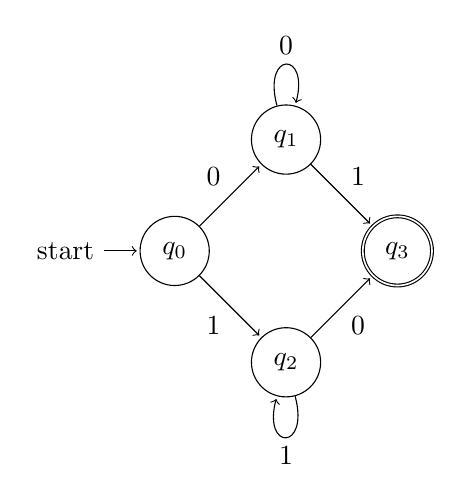
\begin{tikzpicture}[shorten >=1pt,node distance=2cm,on grid,auto] 
   \node[state,initial] (q_0)   {$q_0$}; 
   \node[state] (q_1) [above right=of q_0] {$q_1$}; 
   \node[state] (q_2) [below right=of q_0] {$q_2$}; 
   \node[state,accepting](q_3) [below right=of q_1] {$q_3$};
    \path[->] 
    (q_0) edge  node {0} (q_1)
          edge  node [swap] {1} (q_2)
    (q_1) edge  node  {1} (q_3)
          edge [loop above] node {0} ()
    (q_2) edge  node [swap] {0} (q_3) 
          edge [loop below] node {1} ();
\end{tikzpicture}

\subsection{Finite Automata}

\subsection{Non-finite Automata}

\subsection{Position Automata}

%\chapter{State of the Art}\label{chap:art}
\chapter{State of the Art}\label{chap:art}

\section{Introduction}
Regular expressions (regex) remain one of the most powerful and widely adopted tools for string pattern matching across programming languages, search tools, and data processing pipelines. While their theoretical foundation lies in formal language theory, the practical implementation of regex engines often diverges from the idealized models. This chapter mentions the state of the art in regex engine designs and regex language features, with a particular focus on performance trade-offs, security concerns, and evolving capabilities.

\section{Engine Architectures}
%Regex engines are typically implemented using one of the following architectures:
Regular expressions are most commonly used to look for patterns of strings, known as matching. The basis for this operation are the regular expression engines.
At a high level, regex engines can be grouped by how they traverse the implicit nondeterministic automaton of a pattern. Backtracking engines explore one path at a time, pushing alternative choices on a stack; NFA simulation engines keep all active states in parallel; DFA and hybrid engines trade memory for predictable time; and high-throughput engines emphasize vectorization and streaming.

\subsection{Classic NFA}
The classic backtracking NFA matcher is driven by the pattern: the regular expression acts like a small procedural program that dictates how the engine explores matches and handles failure. The engine begins at the start of the text and attempts to match the pattern from that position; if it fails, it “bumps along,” advancing one character and trying again. Once the first tokens of the pattern match the text, the engine proceeds through the regex. At any choice point—such as an alternation, an optional, or a quantifier—it selects one alternative to try and records the others, together with the current input position. If the chosen path later fails, the engine backtracks to the most recent choice point and resumes with a saved alternative. If all saved alternatives are exhausted, the attempt from that starting position fails and the engine bumps along to the next character.

If the engine reaches the end of the pattern with all constraints satisfied, it declares success and discards any remaining, unexplored alternatives. A key consequence is that the order of alternatives matters: typical backtracking engines implement leftmost-first semantics rather than leftmost-longest, so the first workable alternative can win even if a longer match exists.

Because the engine literally follows the structure of the regex, you control its search by how you write the pattern: place safer or more selective alternatives first, avoid ambiguous constructs under repetition, and structure patterns to minimize backtracking and to fail fast when appropriate.

\subsection{POSIX NFA}
Similarly to the classic NFA engine, the POSIX NFA engine will match in the same way but memorize and continue when a successfull match is found. This is done to see if a longer, leftmost match can be found later on.

\subsection{DFA}
A DFA-based matcher is driven by the input text rather than by the pattern. After compiling the pattern into a deterministic automaton, the engine scans the input once, advancing a single current state per character with no need to branch or revisit earlier positions. Intuitively, each DFA state encodes all viable continuations of the match; this removes the need for backtracking and yields predictable, linear-time behavior in the length of the input (and proportional to the automaton size). In search mode, DFA-style engines are typically implemented to report the leftmost match, and many implementations further return the leftmost-longest match by continuing to advance while remembering the last accepting position. Because the traversal is deterministic, there is no notion of “trying one alternative before another”: the match policy is fixed by the automaton, not by the syntactic order of subexpressions.

This approach is efficient, but it comes with trade-offs. First, you cannot influence the exploration order to emulate backtracking behaviors; the engine will not “prefer” one branch over another, and constructs like atomic groups or possessive quantifiers are largely moot because there is no backtracking to prune. Second, features that go beyond regular languages—most notably backreferences—are not supported in a pure DFA framework, and general look-around assertions are often unavailable or only supported in restricted, regular cases. Third, while matching is fast, precompilation can be more expensive in time and memory due to determinization; in the worst case, the number of DFA states may grow exponentially, which practical systems mitigate with lazy or hybrid techniques. Finally, although some DFA-centric libraries provide submatch extraction using taged automata or similar mechanisms, rich capturing semantics are more limited than in backtracking engines.

\subsection{Hybrid}
Hybrid engines try to take the best of both worlds in both NFAs and DFAs. They perform a depth-first search through the space of matches. At each point of nondeterminism—due to alternation, optional constructs, or unbounded quantifiers—they choose one option to continue and save the others as choice points on an internal stack. If a later step fails, the engine pops a choice point and resumes from there. This approach yields intuitive behavior and supports rich features, including capturing groups, backreferences, and look-around. However, in the presence of ambiguous subpatterns under repetition, the number of explored paths can grow exponentially, making these engines particularly susceptible to ReDoS.

Spencer’s classic backtracking implementation is perhaps the best known and most used, embodying closely the architecture described above. Conceptually, its state comprises the current regex node, the current input index, and a stack of saved alternatives. Consider the pattern \texttt{(a|aa)+\$} against the input \texttt{aaaa\ldots a} without a trailing \texttt{b}. The matcher repeatedly chooses the left alternative \texttt{a}, consuming a single character while saving a choice point for the \texttt{aa} branch at each iteration. At the end of input it fails to satisfy the end anchor, so it begins to backtrack, popping choice points and trying to repartition the run of \texttt{a}s using \texttt{aa} segments. The number of such partitions grows exponentially with the length of the input, and the engine must examine many of them before determining there is no match. This example illustrates how overlapping alternatives inside a quantifier, combined with a terminal failure, can lead directly to catastrophic backtracking.
Great examples of this engine being used widely are the tools GNU egrep and awk.

\section{Feature Sets of Regex Languages}
Regex languages have evolved far beyond classical regular expressions as defined in formal language theory and in general do not correspond to regular languages. The following extensions are now standard in most industrial-strength engines:

\subsection{Backreferences}
Backreferences allow the engine to refer to previously captured groups. This enables matching non-regular patterns (e.g., repeated substrings) and breaks the regular language model.

\subsection{Lookahead and Lookbehind}
These zero-width assertions check what follows or precedes a pattern without consuming input. They are useful for complex validations but add significant complexity.

\subsection{Unicode and Multilingual Support}
Modern engines increasingly support Unicode properties (e.g., \verb|\p{L}| for letters) and normalization, essential for multilingual applications.

\subsection{Named Capture Groups and Subroutines}
Named groups (\verb|(?<name>...)|) and recursive subpatterns (e.g., \verb|(?R)|) have become essential for advanced pattern extraction.

\subsection{Flags and Modes}
Regex engines support flags for case insensitivity, multiline matching, dot-all mode (where \verb|.| matches newlines), and others.

\section{Engines and Libraries}
\subsection{RE2}
Developed by Google, RE2 is a DFA-based engine designed to never exceed linear time or memory. It disallows features like backreferences for safety and predictability. 
%https://swtch.com/~rsc/regexp/regexp1.html

\subsection{PCRE2}
An industry-standard library used in PHP and many scripting tools. It supports extensive features including backtracking control verbs and recursive patterns. %https://github.com/PCRE2Project/pcre2

\subsection{Hyperscan}
Hyperscan is Intel’s regular expression matching engine, designed specifically for high-throughput and low-latency applications. It serves as a core component in several security and networking tools, including intrusion detection systems like Suricata and firewalls.

Traditional regex engines (e.g., backtracking-based ones like PCRE) often struggle with performance bottlenecks due to their sequential nature and vulnerability to ReDoS attacks. Hyperscan addresses these limitations by combining multiple automata models—particularly NFAs and DFAs—with a hybrid execution strategy that leverages Single Instruction, Multiple Data (SIMD) parallelism and tiled execution on modern CPUs .

According to Wang et al. (\cite{hyperscan}), Hyperscan divides regexes into multiple subgraphs, such as anchored DFAs for simple patterns and NFAs for complex constructs. This hybrid approach enables it to process large volumes of data streams efficiently without the exponential-time risks associated with backtracking engines.

However, as also noted in \cite{hyperscan}, Hyperscan will also enforce syntactic restrictions when compiling. Regexes that are deemed vulnerable or ambiguous are rejected, therefore limiting expressiveness and versatility, especially when the user is looking for nested repetition (e.g. $(a+)+$, looking to match one or more of one or more $a$'s) or greedy alternation (e.g. $(a|aa)+$, matching a sequence of $a$ or $aa$, repeated, resulting in three matches for a string such as $aa$).

\subsection{Rust's \texttt{regex} Crate}
Implements a hybrid DFA/NFA model and guarantees linear-time performance by excluding features like backreferences.

\section{Prevalency of ReDoS and solutions}
\subsection{Revealer}
Mention the revealer paper here!
%https://seclab.cse.cuhk.edu.hk/papers/sp21_redos.pdf

\section{Reluctance}
If it works...

\chapter{Counting}\label{chap:counting}
In this chapter, we will explore the concept of counting in the context of formal languages and automata theory as well as explain the implementation for fixed and bounded repetition in FAdo.

\section{Counting in Formal Languages}
In formal language theory, counting refers to the ability of a language or an automaton to enforce numeric constraints over the number of symbols or patterns within strings. Specifically, it deals with the ability to recognize whether certain elements occur a specified number of times—or in a specific numerical relationship to others.
Current tools are already able to do this, including some non-backtracking matchers.

\section{Derivatives of operations in Extended Regular Expressions} %TODO: CHANGE THIS
Given a word $w = xyz$ and a regular expression $\alpha$, $w \in L(\alpha)$ if $\varepsilon(d_w(\alpha)) = \varepsilon$.
In order to match with fixed and bounded repetition, one must first solve the derivatives for those operations.

\begin{thm}
	Given $e \in RegExp(\Sigma)$, the following holds:
	\begin{align*}
		\varepsilon(e) + e = e
	\end{align*}
\end{thm}
\begin{proof}
	Let $e \in RegExp(\Sigma)$. The proof is by iterating through both possible scenarios where $\varepsilon \in L(e)$ and $\varepsilon \notin L(e)$.
	For $\varepsilon \in L(e)$, we have that $\varepsilon(e) = \varepsilon$. And so,
	\begin{align*}
		& \varepsilon(e) + e = e \\
		& \Rightarrow \varepsilon + e = e \\
		& \Rightarrow e = e
	\end{align*}
	holds. On the other hand, for $\varepsilon \notin L(e)$, we have that $\varepsilon(e) = \emptyset$. Therefore,
	\begin{align*}
		& \varepsilon(e) + e = e \\
		& \Rightarrow \emptyset + e = e \\
		& \Rightarrow e = e
	\end{align*}
	also holds.
\end{proof}

\subsection{Fixed Repetition}
For a fixed repetition, we need $r$ to occur $n$ times, resulting in the notion $r^n$.
% PROOF
%\begin{thm}
%	Given $e \in RegExp(\Sigma)$ and $n \in \Npos$, we have that
%	\begin{align*}
%		d_a(e^n) = d_a(e)e^{n-1}
%	\end{align*}
%	is true.
%\end{thm}
%\begin{proof}
%	Let $e \in RegExp(\Sigma)$ and $n \in \Npos$. The following holds:
%	\begin{align*}
%		d_a(e) = d_a(e)e^0 = d_a(e)
%	\end{align*}
%	We can also suppose that
%	\begin{align*}
%		d_a(e^{n-1}) = d_a(e)e^{n-2}
%	\end{align*}
%	And so, we can use the results above to do the following:
%	\begin{align*}
%		d_a(e^n) &= d_a(ee^{n-1}) \\
%		&= d_a(e)e^{n-1} + \varepsilon(e)d_a(e^{n-1}) \\
%		&= d_a(e)e^{n-1} + \varepsilon(e)d_a(e)e^{n-2} \\
%		&= (d_a(e)e + \varepsilon(e)d_a(e))e^{n-2} \\
%		&= (d_a(e)(e+\varepsilon(e)))e^{n-2} \\
%		&= d_a(e)e^{n-1}
%	\end{align*}
%\end{proof}
\begin{thm}
	\label{thm:fixed_repetition_derivative}
	Given $e \in RegExp(\Sigma)$ and $n \in \Npos$, we have:
	\begin{align*}
		d_a(e^n) = d_a(e)\,e^{n-1}.
	\end{align*}
\end{thm}

\begin{proof}
	We proceed by induction on $n \in \Npos$. For the base case \( n = 1 \),
	\begin{align*}
		d_a(e^1) = d_a(e) = d_a(e)e^0 = d_a(e)\varepsilon = d_a(e).
	\end{align*}
	Since the identity holds for \(n = 1\), lets assume that the identity holds for some \(n-1 \geq 1\), i.e.,
	\begin{align*}
		d_a(e^{n-1}) = d_a(e)e^{n-2}.
	\end{align*}
	We want to show it holds for \(n\). Using the product rule:
	\begin{align*}
		d_a(e^n) &= d_a(ee^{n-1}) \\
		&= d_a(e) e^{n-1} + \varepsilon(e) d_a(e^{n-1}) \\
		&= d_a(e) e^{n-1} + \varepsilon(e) d_a(e) e^{n-2} \\
		&= d_a(e) \left(e^{n-1} + \varepsilon(e) e^{n-2}\right) \\
		&= d_a(e) \left(ee^{n-2} + \varepsilon(e) e^{n-2}\right) \\
		&= d_a(e) (e + \varepsilon(e))e^{n-2} \\
		&= d_a(e) e^{n-1}.
	\end{align*}
	This completes the induction.
\end{proof}

As an example, let $r = ab$ such that $r^2 = abab$. Replacing with the theorem above:
\begin{align*}
	d_a(r^2) &= d_a(r \cdot r) \\
	&= d_a(abab)  \\
	&= d_a(a)bab + d_a(bab) \\
	&= \varepsilon bab + \emptyset \\
	&= bab
\end{align*}

% ADD e^n results for n=0, n=1 and n>1

\subsection{Bounded Repetition}
Supplementing the fixed repetition notion, we now add a maximum bound so that $r$ can occur at least $n$ times and at maximum $m-1$ times: $r^{n,m}$.

\begin{thm}
	Given $e \in RegExp(\Sigma)$, $n \in \Npos$, $m > n$, and $a \in \Sigma$, we have:
	\begin{align*}
		d_a(e^{n,m}) =
		\begin{cases}
			d_a(e) e^{n-1,m-1}, & \text{if } n > 1, \\
			d_a(e) + d_a(e) e^{1,m-1}, & \text{if } n = 1.
		\end{cases}
	\end{align*}
\end{thm}

\begin{proof}
	Let $e \in RegExp(\Sigma)$ and let $n, m \in \Npos$ with $m > n$. By definition of bounded iteration:
	\begin{align*}
		e^{n,m} &= \sum_{i=n}^{m} e^i,
	\end{align*}
	and by the linearity of derivatives over sums:
	\begin{align*}
		d_a(e^{n,m}) &= \sum_{i=n}^{m} d_a(e^i).
	\end{align*}
	Using the known identity $d_a(e^i) = d_a(e) e^{i-1}$, we have:
	\begin{align*}
		d_a(e^{n,m}) &= \sum_{i=n}^{m} d_a(e) e^{i-1} \\
		&= d_a(e) \sum_{i=n}^{m} e^{i-1}.
	\end{align*}
	Letting $j = i - 1$, this becomes:
	\begin{align*}
		d_a(e^{n,m}) &= d_a(e) \sum_{j=n-1}^{m-1} e^j = d_a(e) e^{n-1,m-1}.
	\end{align*}
	Considering both cases, for $n > 1$, the expression is already in its final form:
	\begin{align*}
		d_a(e^{n,m}) = d_a(e) e^{n-1,m-1}.
	\end{align*}
	And for $n = 1$, we have:
	\begin{align*}
		d_a(e^{1,m}) &= d_a(e) e^{0,m-1} \\
		&= d_a(e) + d_a(e) e^{1,m-1}.
	\end{align*}
	This completes the proof.
\end{proof}
Furthermore, we can include the infinite upper bound: $r^{n,\infty}$.
\begin{align*}
	r^{n,\infty} = r^nr^\star
\end{align*}
We can simplify it even more, depending on the value of $n$. Assuming $n=0$:
\begin{align*}
	r^{0,\infty} = r^0r^\star = \varepsilon r^\star =  r^\star
\end{align*}
Lastly, for $n=1$:
\begin{align*}
	r^{1,\infty} = r^1r^\star = rr^\star =  r^+
\end{align*}

\begin{thm}
	Given $e \in RegExp(\Sigma)$, $n \in \N$ and $a \in \Sigma$, we have:
	\begin{align*}
		d_a(e^{n,\infty}) =
		\begin{cases}
			d_a(e)e^{n-1}e^\star, & \text{if } n>0, \\
			d_a(e)e^*, & \text{otherwise}.
		\end{cases}
	\end{align*}
\end{thm}
\begin{proof}
	Let $e \in RegExp(\Sigma)$, $n \in \N$, and $a \in \Sigma$. We have,
	\begin{align*}
		d_a(e^{n,\infty}) &= d_a(e^ne^\star) \\
		&= d_a(e^n)e^\star. %\\
%		\intertext{using \ref{thm:fixed_repetition_derivative}:}
%		&= d_a(e)e^{n-1}e^\star
	\end{align*}
	Now, if $n>0$, we can use \ref{thm:fixed_repetition_derivative}:
	\begin{align*}
		d_a(e^n)e^\star &= d_a(e)e^{n-1}e^\star.
	\end{align*}
	Otherwise, if $n=0$, we can just replace accordingly:
	\begin{align*}
		d_a(e^ne^\star) = d_a(e^0e^\star) = d_a(e^*) = d_a(e)e^*.
	\end{align*}
	This concludes the proof.
\end{proof}
For instance, given $r = ab$ such that $r^2 = abab$ and $r^3 = ababab$, we have:
\begin{align*}
	d_a(r^{[2,4[}) &= d_a(abab) + d_a(ababab) \\
	&= d_a(abab) + d_a(ababab) \\
	&= d_a(a)bab + d_a(bab) + d_a(a)babab + d_a(babab) \\
	&= \varepsilon bab + \emptyset + babab + \emptyset \\
	&= bab + babab.
\end{align*}
Extending to the infinity case, $r^{[2, \inf[}$:
\begin{align*}
	d_a(r^{[2,\inf[}) &= d_a(abab) + d_a((ab)^*) \\
	&= d_a(a)bab + d_a(bab) + d_a(ab)\cdot(ab)^* \\
	&= \varepsilon bab + \emptyset + (d_a(a)b + d_a(b)) \cdot (ab)^* \\
	&= bab + (\varepsilon b + \emptyset) \cdot (ab)^* \\
	&= bab + b(ab)^*.
\end{align*}

%For instance, if $m = 2$, we have that $r^{[2, \inf[}$

%The regular expression $r^{[2, \inf[}$ will match any $(ab)^k$ with $k \geq 2$.

%Given $w = abababab$ and $m = 2$,  will match 

%The string $abababab$ can be matched by $r^{[2, \inf[}$

%\begin{thm}
%	Given $e \in RegExp(\Sigma)$, $n \in \Npos$ and $m>n$, we have that
%	\begin{align*}
%	%	d_a(e^{n,m}) = d_a(e) e^{n-1,m-1}
%	d_a(e^{n,m}) = \begin{cases}
%		d_a(e)e^{n-1,m-1} & n>1 \\
%		d_a(e)+(d_a(e))e^{1,m-1} & n=1
%	\end{cases}
%	\end{align*}
%	is true.
%\end{thm}
%\begin{proof}
%	Let $e \in RegExp(\Sigma)$. We first need to simplify the main expression:
%	\begin{align*}
%		d_a(e^{n,m}) &= \sum_{i=n}^{m} d_a(e^i) \\
%		&= \sum_{i=n}^{m} (d_a(e))e^{i-1} \\
%		&= d_a(e) \sum_{j=n-1}^{m-1} e^j \\
%		&= d_a(e) e^{n-1,m-1}
%	\end{align*}
%	Thus, for $n=1$, we have that
%	\begin{align*}
%		d_a(e^{n,m}) &= d_a(e)e^{0,m-1} \\
%		&= d_a(e) + (d_a(e))e^{1,m-1}
%	\end{align*}
%	And lastly, for $n>=1$ we have that
%	\begin{align*}
%		d_a(e^{n,m}) &= (d_a(e))e^{n-1,m-1}
%	\end{align*}
%\end{proof}

%For instance, if $m = 2$, we have that $r^{[2, \inf[}$

%The regular expression $r^{[2, \inf[}$ will match any $(ab)^k$ with $k \geq 2$.

%Given $w = abababab$ and $m = 2$,  will match 

%The string $abababab$ can be matched by $r^{[2, \inf[}$


\section{Implementation in FAdo}
In order to implement these new syntactic constructs of extended regular expressions in FAdo, we added exact-power and counted-repetition nodes to the regular expression abstract syntax tree and define their derivatives, partial derivatives and linear form cases.

\subsection{CPower}
\textit{CPower} is the class responsible for the construction of regular expressions using the fixed repetition operator.

\begin{lstlisting}[language=Python]
class CPower(Unary):
	def __init__(self, arg, n, sigma=None):
	self.arg = arg
	self.n = n
	self.Sigma = sigma
	self._ewp = False if self.n > 0 else True
	
	...
\end{lstlisting}

As shown above, the class inherits from the \textit{Unary}, which only defines the \textit{Unary.Sigma} and \textit{Unary.arg} properties, letting the class hold a alphabet set (representing $\Sigma$) and the symbol used to construct this operator.

In order to integrate the class fully with \textit{FAdo}, some more methods had to be implemented.

\begin{lstlisting}[language=Python]
	def linearForm(self):
		arg_lf = self.arg.linearForm()
		lf = dict()
		for head in arg_lf:
			lf[head] = set()
			for tail in arg_lf[head]:
				lf[head].add(self.derivative(head))
		return lf

	def partialDerivatives(self, sigma):
		return self.arg.partialDerivatives(sigma)
	
	def derivative(self, sigma):
		if str(sigma) in str(self.Sigma):
			if self.n == 0:
				return CEmptySet(sigma)
			elif self.n == 1:
				return self.arg.derivative(sigma)
			else:
				return CConcat(self.arg.derivative(sigma), CPower(self.arg, self.n-1, self.Sigma))
		else:
			return CEmptySet(sigma)
\end{lstlisting}

\subsection{CCount}
\textit{CCount} is the class responsible for the construction of regular expressions using the bounded repetition operator.


\begin{lstlisting}[language=Python]
	class CCount(Unary):
		def __init__(self, arg, min, max = None, sigma = None):
			self.arg = arg
			self.min = int(min)
			self.max = "inf" if max == -1 or max == "inf" else int(max)-1
			self.Sigma = sigma
	
			if self.min==0:
				self._ewp = True
\end{lstlisting}

As shown above, and much like \textit{CPower}, the class also inherits from \textit{Unary}. The constructor adjusts the bounds accordingly and sets the empty word property based on whether the minimum repetition is zero.

To fully integrate the class with \textit{FAdo}, several methods are implemented, including string representation, partial derivatives, linear form computation, and marking functions:

\begin{lstlisting}[language=Python]
	def derivative(self, sigma):
		if str(sigma) in str(self.Sigma):
			if self.max == "inf" or self.max == None:
				if self.min == 0:
					return CConcat(self.arg.derivative(sigma), CStar(self.arg, self.Sigma))
				else:
					return CConcat(self.arg.derivative(sigma), CCount(self.arg, self.min-1, self.max, sigma), self.Sigma)
			else:
				if self.max > 1:
					if self.min == 0:
						return CConcat(self.arg.derivative(sigma), CCount(self.arg, self.min, int(self.max), self.Sigma))
					else:
						return CConcat(self.arg.derivative(sigma), CCount(self.arg, self.min-1, int(self.max), self.Sigma))
				elif self.max == 1:
					return self.arg.derivative(sigma)
				else:
					CEpsilon(sigma)
		else:
			return CEmptySet(sigma)
		
	def partialDerivatives(self, sigma):
		arg_pdset = self.arg.partialDerivatives(sigma)
		pds = set()
		for pd in arg_pdset:
			if pd.emptysetP():
				pds.add(CEmptySet(self.Sigma))
			elif pd.epsilonP():
				pds.add(self)
			else:
				pds.add(CConcat(pd, self, self.Sigma))
		return pds
\end{lstlisting}

The \texttt{linearForm} method is exactly the same as \texttt{CPower}'s.

%\begin{lstlisting}[language=Python]
%	def linearForm(self):
%		arg_lf = self.arg.linearForm()
%		lf = dict()
%		for head in arg_lf:
%			lf[head] = set()
%			for tail in arg_lf[head]:
%				lf[head].add(self.derivative(head))
%		return lf
%\end{lstlisting}

\subsection{Grammar}
For ease of use and protoyping, we utilized \textit{FAdo}'s ability to parse a regular expression using a common Python \textit{string}. To do this, \textit{FAdo} utilizes a library called Lark. Lark is a modern, fast and flexible parsing toolkit for Python that supports both LALR(1) and Earley parsers, enabling the parsing of all context-free grammars with features like EBNF, AST generation, and grammar composition \cite{lark_parser}.
The new grammar can be seen in \ref{appendix:regexp_lark} and the most notable changes are the following:
\begin{lstlisting}
	| rep _CARET _LEFBR digit _RIGBR -> pow_min
	| rep _CARET _LEFBR digit _COMMA digit _LEFBR -> pow_minmax
	| rep _CARET _LEFBR digit _COMMA _INFTY _LEFBR -> pow_inf
\end{lstlisting}
These rules (along with some more utilitary definitions such as the \texttt{\_LEFBR} and \texttt{\_RIGBR}, which are the symbols '\texttt{\string[}' and '\texttt{\string]}') will route the following cases (code in Appendix \ref{appendix:regexp_builders}):
\begin{itemize}
	\item \textbf{pow\_min}: For the cases $r^{n}$ and $r^{n,\infty}$, where $r \in RegExp(\Sigma)$ and $n \in \Npos$
	\item \textbf{pow\_minmax}: For the case $r^{n,m}$, where $r \in RegExp(\Sigma)$ and $n \in \Npos, m>n$
	\item \textbf{pow\_inf}: Calls \textit{pow\_min} with a special argument that selects the infinity case
\end{itemize}

\section{Single Matching}
When referring to matching in the context of regular expressions, one typically means simply determining whether a given word is a member of the language defined by a specific regular expression.
We can define this problem formally as:
\begin{defn}
	\label{defn:single_matching}
	Given $e \in RegExp(\Sigma)$ and a word $w \in \Sigma^\star$, we say that $w$ matches $e$ if $w \in L(e)$.
\end{defn}

To look for matches using \textit{FAdo}, we first need to choose a regular expression. For the sake of this example, let $r = ab + ba$. Informally, this regular expression will match any $ab$ or $ba$ character sequences in an input text. To do this, we first need to import the grammar using Lark and parse the regular expression to get a parsed syntax tree. With this tree, we can use \textit{FAdo}'s \texttt{BuildRegexp} class and invoke its \texttt{transform} method, which will iteratively transform each of the trees nodes into abstract \textit{FAdo} class objects:
\begin{lstlisting}[language=Python]
	r = "ab+ba"
	regGrammar = lark.Lark.open("lang/regexp_test.lark", start="rege", parser="lalr")
	tree = regGrammar.parse(r)
	reg : RegExp = BuildRegexp(context={"sigma": None}).transform(tree)
	reg.setSigma(reg.setOfSymbols())
\end{lstlisting}
We now have a regular expression object. We can use it to build a DFA using Brzozowski's derivatives construction:
\begin{lstlisting}[language=Python]
	dfa_z = reg.dfaBrzozowski()
\end{lstlisting}
Finally, having a DFA object, we can then use the \texttt{evalWordP} function to verify if $w \in L(r)$ for a given $w \in \Sigma^\star$, which can be, for this example, $w = ab$:
\begin{lstlisting}[language=Python,label={code:eval_word_dfa}]
	w = "ab"
	if dfa_z.evalWordP(w):
		print("w belongs to the language of r")
	else:
		print("w does not belong to the language of r")
\end{lstlisting}
With the result being:
\begin{lstlisting}[language=Python]
	w belongs to the language of r
\end{lstlisting}
We can do the exact same with the new syntax. Let $r = (ab)^{1,3}$. First, parse the regular expression and display it:
\begin{lstlisting}[language=Python]
	r = "(ab)^[1,3["
	tree = regGrammar.parse(r)
	reg : RegExp = BuildRegexp(context={"sigma": None}).transform(tree)
	reg.setSigma(reg.setOfSymbols())
	dfa_z = reg.dfaBrzozowski()
	dfa_z.display()
\end{lstlisting}

\begin{figure}[H]
	\centering
	\begin{tikzpicture}[shorten >=1pt,node distance=2cm,on grid, auto,initial text=]
		
		% --- States ---
		\node[state, initial] (q0) {0};
		\node[state]          (q1) [above right=of q0] {1};
		\node[state]          (q2) [below right=of q0] {2};
		\node[state, accepting]         (q3) [right=22mm of q1] {3};
		\node[state]          (q4) [right=22mm of q2] {4};
		\node[state]          (q5) [above right=of q3] {5};
		\node[state]          (q6) [right=20mm of q3] {6};
		\node[state, accepting]         (q7) [right=22mm of q6] {7};
		\node[state]          (q8) [right=22mm of q7] {8};
		
		% --- Transitions ---
		\path[->]
		(q0) edge node {$b$} (q1)
		edge[swap] node {$a$} (q2)
		
		(q1) edge[loop above] node {$b, a$} ()
		
		(q2) edge node {$b$} (q3)
		edge[swap] node {$a$} (q4)
		
		(q4) edge[loop below] node {$b, a$} ()
		
		(q3) edge node {$b$} (q5)
		edge[swap] node {$a$} (q6)
		
		(q5) edge[loop above] node {$b, a$} ()
		
		(q6) edge node {$b$} (q7)
		edge[bend right=40, swap] node {$a$} (q8)
		
		(q7) edge node {$b, a$} (q8)
		
		(q8) edge[loop right] node {$b, a$} ();
	\end{tikzpicture}
	\caption{Diagram of the DFA built using Brzozowski's method for the regular expression $r = (ab)^{1,3}$.}
	\label{fig:dfa_brzozowski_counting}
\end{figure}
Then, try to match $w = ab$ using the same code from \ref{code:eval_word_dfa}, which yields the following:
\begin{lstlisting}[language=Python]
	w belongs to the language of r
\end{lstlisting}
Trying again with a text that does not match, $w = ababab$, yields:
\begin{lstlisting}[language=Python]
	w does not belong to the language of r
\end{lstlisting}
%Formally, .

\chapter{Matching}\label{chap:matching}
% Matching is used to search, validate, or extract parts of text based on these patterns. For example, a regex can be used to find all dates in a document or to ensure a password meets certain rules.

Regex \emph{matching} is the process of checking whether a piece of text fits a specific pattern described using a regular expression (regex). A regex is a compact, rule-based way to describe sets of strings—like email addresses, phone numbers, or specific word formats.

In this chapter, we will discuss the different approaches to matching regular expressions, the implications of using them, and the performance considerations that arise from these choices. Furthermore, we will also present a novel approach based on position automata, which aims to mitigate the performance issues associated with traditional regex engines while preserving some of the extended expressiveness of regex patterns.

\section{Modified Position Automata}
A \emph{position automaton} is a type of nondeterministic finite automaton (NFA) that facilitates overlapped matching.

\begin{algorithm}[H]
\caption{\textsc{nfaPosCount}($R$): Construct Special Position Automaton}
\label{alg:nfaPosCount}
\begin{small}
\begin{algorithmic}[1]
\Require Regular expression $R$
\Ensure NFA $A$

\State $A \gets$ new empty NFA
\State $i \gets A.\text{addInitialState}()$
\State $A.\text{addTransitionStar}(i, i)$ \Comment{Accept any symbol from $\Sigma$}

\State $f_R \gets R.\text{marked}()$
\State $\text{stack} \gets$ empty stack
\State $\text{addedStates} \gets$ empty map

\ForAll{$p \in First(f_R)$}
    \State $q \gets A.\text{addState}(p)$
    \State $\text{addedStates}[p] \gets q$
    \State $\text{stack}.\text{push}((p, q))$
    \State $A.\text{addTransition}(i, p, q)$
\EndFor

% \State $\text{FollowSets} \gets Follow(f_R)$

\While{stack is not empty}
    \State $(s, s_{\text{idx}}) \gets \text{stack}.\text{pop}()$
    \ForAll{$t \in Follow(f_R, s)$}
        \If{$t \in \text{addedStates}$}
            \State $q \gets \text{addedStates}[t]$
        \Else
            \State $q \gets A.\text{addState}(t)$
            \State $\text{addedStates}[t] \gets q$
            \State $\text{stack}.\text{push}((t, q))$
        \EndIf
        \State $A.\text{addTransition}(s_{\text{idx}}, t, q)$
    \EndFor
\EndWhile

\State $e \gets A.\text{addState}()$
\State $A.\text{addTransitionStar}(e, e)$

\ForAll{$p \in f_R.\text{Last}()$}
    \If{$p \in \text{addedStates}$}
        \State $A.\text{addFinal}(\text{addedStates}[p])$
        \State $A.\text{addTransitionStar}(\text{addedStates}[p], e)$
    \EndIf
\EndFor

\end{algorithmic}
\end{small}
\end{algorithm}

\section{Automata-Based Matching}

Given a regular expression $R$, one can construct an NFA $A$ such that $L(A) = L(R)$. Matching then reduces to verifying whether the automaton $A$ accepts the input string $s$. In DFA-based engines, each character of the input leads to a deterministic transition from one state to another, resulting in a guaranteed linear-time match. In contrast, NFA-based engines may involve branching paths due to nondeterminism and can require simulating multiple transitions concurrently.

% \section{Backtracking and Performance Implications}

% Many practical regular expression engines (such as those in Java, Perl, and Python) implement matching using \emph{backtracking}, which simulates an NFA by exploring all possible paths through the automaton recursively. While this allows support for rich and flexible patterns, it can introduce performance issues in certain cases. In particular, patterns with nested or ambiguous quantifiers may cause excessive backtracking, leading to exponential runtime in the worst case—a phenomenon known as \emph{regular expression denial of service} (ReDoS).

For example, consider the following regex pattern:
\begin{verbatim}
	^(a+)+$
\end{verbatim}

\section {Matching with the Modified Position Automaton}
One can find all matches over an input string by constructing the modified position automaton from a regular expression and then simulating the automaton's transitions over the input string. The algorithm presented in this section is designed to track the start and end positions of all matches, including overlapping ones, without relying on backtracking.

\begin{algorithm}[H]
\caption{\textsc{tableMatcher}$(A, s)$: Modified Position Automaton Multi-matcher}
\label{alg:table-matcher}
\begin{small}
\begin{algorithmic}[1]
\Require $A = (\Sigma, Q, \delta, I, F)$: NFA
\Require $s$: input string
\Ensure $M$: mapping from final states to lists of match positions

\State $symbols \gets$ list with $\varepsilon$ prepended to $s$
\State $currentRow \gets$ empty map from states to list of position pairs
\State $finalMatches \gets$ empty map from states to list of matches
\State $position \gets 0$

\ForAll{$sym$ in $symbols$}
    \If{$sym = \varepsilon$}
        \ForAll{$q_0 \in I$}
            \State $currentRow[q_0] \gets [(0, 0)]$
        \EndFor
    \Else
        \State $nextRow \gets$ empty map
        \If{$sym \in \Sigma$}
            \ForAll{$q \in$ \textbf{keys}($currentRow$)}
                % \State $transitions \gets \delta(q, sym)$
                \If{$|\delta(q, sym)| > 0$}
                    \ForAll{$q' \in \delta(q, sym)$}
                        \ForAll{$(start, \_) \in currentRow[q]$}
                            \If{$q' = q$ and $q' \in I$}
                                \State append $(position, position)$ to $nextRow[q']$
                            \Else
                                \State append $(start, position)$ to $nextRow[q']$
                                \If{$q' \in F$}
                                    \State append $(start, position)$ to $finalMatches[q']$
                                \EndIf
                            \EndIf
                        \EndFor
                    \EndFor
                \EndIf
            \EndFor
        \Else
            \Comment{Symbol not in $\Sigma$; treat as fresh start}
            \ForAll{$q_0 \in I$}
                \State $nextRow[q_0] \gets [(position, position)]$
            \EndFor
        \EndIf
        \State $currentRow \gets nextRow$
        \State $position \gets position + 1$
    \EndIf
\EndFor
\State \Return $finalMatches$
\end{algorithmic}
\end{small}
\end{algorithm}

\clearpage

As an example, consider the following regular expression $R$ and input string $w$:
\begin{center}
	$R = (aa+aaa)(aaa+aa)$ \break
	$w = aaaaabaaaaa$
\end{center}

The Glushkov automaton construction for $R$ is as follows:

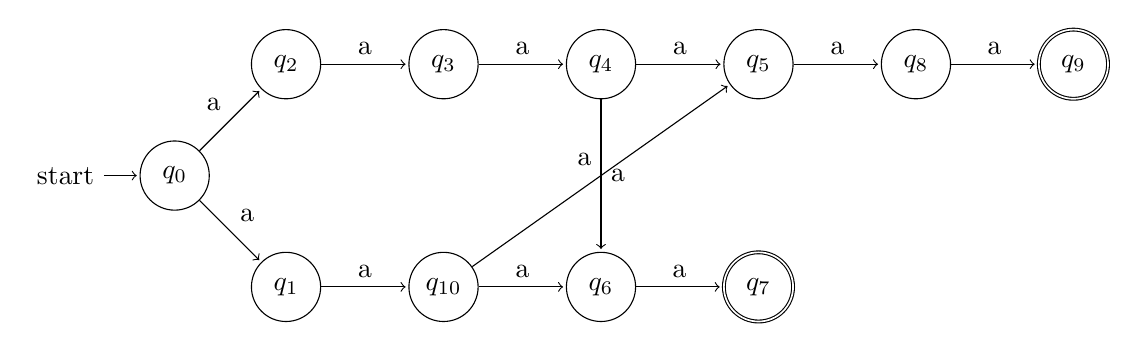
\begin{tikzpicture}[shorten >=1pt,node distance=2cm,on grid, auto]
	\node[state, initial] (q0) {$q_0$};
	\node[state] (q2) [above right=of q0] {$q_2$};
	\node[state] (q3) [right=of q2] {$q_3$};
	\node[state] (q4) [right=of q3] {$q_4$};
	\node[state] (q5) [right=of q4] {$q_5$};
	\node[state] (q8) [right=of q5] {$q_8$};
	\node[state,accepting] (q9) [right=of q8] {$q_9$};

	\node[state] (q1) [below right=of q0] {$q_1$};
	\node[state] (q10) [right=of q1] {$q_{10}$};
	\node[state] (q6) [right=of q10] {$q_6$};
	\node[state,accepting] (q7) [right=of q6] {$q_7$};

	\path[->]	(q0)	edge	node	{a} (q1)
						edge	node	{a} (q2)
				(q1)	edge	node	{a} (q10)
				(q10)	edge	node	{a} (q6)
				(q10)	edge	node	{a} (q5)
				(q6)	edge	node	{a} (q7)
				(q2)	edge	node	{a} (q3)
				(q3)	edge	node	{a} (q4)
				(q4)	edge	node	{a} (q5)
				(q4)	edge	node	{a} (q6)
				(q5)	edge	node	{a} (q8)
				(q8)	edge	node	{a} (q9);
\end{tikzpicture}

Meanwhile, the modified position automaton for this regular expression can be constructed using the algorithm presented in \ref{alg:nfaPosCount}, resulting in the following:

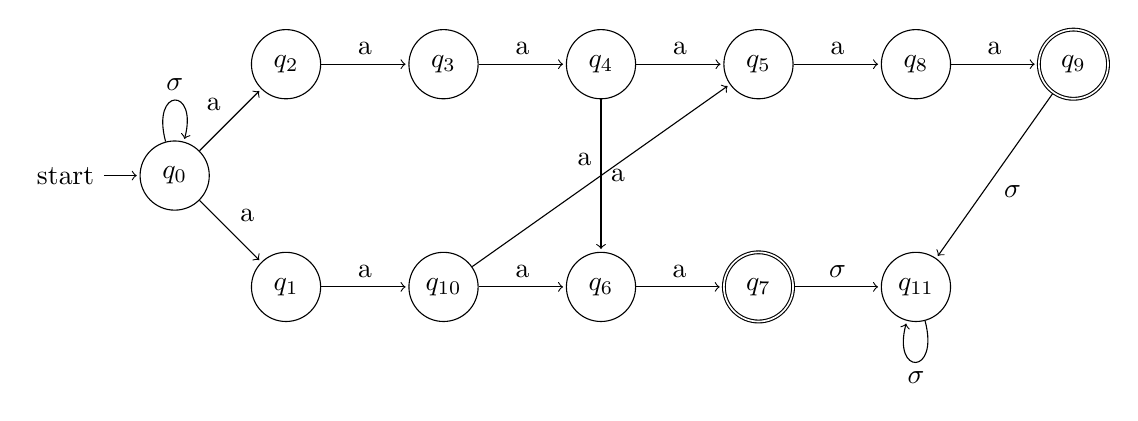
\begin{tikzpicture}[shorten >=1pt,node distance=2cm,on grid, auto]
	\node[state, initial] (q0) {$q_0$};
	\node[state] (q2) [above right=of q0] {$q_2$};
	\node[state] (q3) [right=of q2] {$q_3$};
	\node[state] (q4) [right=of q3] {$q_4$};
	\node[state] (q5) [right=of q4] {$q_5$};
	\node[state] (q8) [right=of q5] {$q_8$};
	\node[state,accepting] (q9) [right=of q8] {$q_9$};

	\node[state] (q1) [below right=of q0] {$q_1$};
	\node[state] (q10) [right=of q1] {$q_{10}$};
	\node[state] (q6) [right=of q10] {$q_6$};
	\node[state,accepting] (q7) [right=of q6] {$q_7$};

	\node[state] (q11) [below right=of q9,right=of q7] {$q_{11}$};

	\path[->]	(q0)	edge	node	{a} (q1)
						edge	node	{a} (q2)
						edge [loop above] node {$\sigma$} ()
				(q1)	edge	node	{a} (q10)
				(q10)	edge	node	{a} (q6)
				(q10)	edge	node	{a} (q5)
				(q6)	edge	node	{a} (q7)
				(q7)	edge	node	{$\sigma$} (q11)
				(q2)	edge	node	{a} (q3)
				(q3)	edge	node	{a} (q4)
				(q4)	edge	node	{a} (q5)
				(q4)	edge	node	{a} (q6)
				(q5)	edge	node	{a} (q8)
				(q8)	edge	node	{a} (q9)
				(q9)	edge	node	{$\sigma$} (q11)
				(q11)	edge [loop below] node {$\sigma$} ();
\end{tikzpicture}

One can then apply the matching algorithm (\ref{alg:table-matcher}) to an input string, resulting in the following match table:


% When we apply the matching algorithm (\ref{alg:table-matcher}) to an input string, it will traverse the automaton and record all positions where matches occur. This approach ensures that we can find all possible matches, including those that overlap, without falling into the exponential blowup trap of backtracking.

%\chapter{Resultados e análise}\label{chap:results}
% !TEX root = thesis.tex

\chapter{Results and Discussion}\label{chap:results}

This is a test


\section{Algorithm Analysis}

\section{Accuracy}

The methods of evaluating

\section{Comparison with Other Methods}

\section{Examples}
 

%\chapter{Conclusões}\label{chap:conc}
\chapter{Conclusion}
In this work, we contribute with a new approach to address the problem of \ac{ReDoS}, focusing on a solution outside of traditional backtracking engines.
We explored the underlying causes of ReDoS vulnerabilities, particularly how certain finite automaton evaluators can lead to catastrophic performance, due to the deviation of the path of theory. To tackle this, we extended \textit{FAdo} to support fixed and bounded repetition operators. To recognize this new grammar, the default Lark grammar present in \textit{FAdo} was modified. The new type of automaton is capable of performing multiple overlapping matching. In security analysis, for instance, this means that one can find all possible malicious substrings in payloads (e.g., nested injection markers), because attack signatures can overlap and/or nest. Another example is the efficient search for DNA protein patterns, where biological sequences often contain repeating and/or nested patterns.

Most of the examples (regular expression pattern datasets) we found for this work did not include overlapping. The only way to do so (that we know of, currently implemented in state-of-the-art languages) is using \texttt{lookahead} assertions, and even this strategy does not work well, since they are expensive and hard to read. As a result, limited validation data exists for evaluating overlapping matchers, which makes empirical comparison with other state-of-the-art techniques challenging.

Anyhow, this work contributes towards safer and more predictable regular expression evaluation by combining formal methods and a new matching strategy.

Future work may turn towards making these algorithms more efficient by switching to a different language or integrating them into a larger ecosystem.
It would also be valuable to develop tools capable of automatically generating text datasets with overlapping patterns for benchmarking and evaluation.

%With this, a new type of automaton was implemented and used to perform multiple overlapping matching.



%% references
%\renewcommand{\bibname}{Referências} % o babel portuguese coloca Bibliografia
% os meses do ficheiro bib poderão aparecer em inglês, caso se pretenda deve-se colocar o texto em português explicitamente no ficheiro bid
\cleardoublepage%
\phantomsection%
\printbibliography[heading=bibintoc]%


%% appendix
\appendix
\include{appendix/appendix1}

%% bye
\end{document}
